\pdfminorversion=5
\documentclass[unnumsec,webpdf,contemporary,large]{oup-authoring-template}

\usepackage{graphicx}
\usepackage{url}
\usepackage{microtype}

% Long URLs in the Data availability section must break inside the column
% rather than run into the margin.
\usepackage{xurl}

% The class calls \societylogo{} in its running head but only ships it
% commented out, which aborts the build at the first \section.
\providecommand{\societylogo}{}

\begin{document}

\journaltitle{Bioinformatics}
\copyrightyear{2026}
\pubyear{2026}
\appnotes{Application Note}
\firstpage{1}

\title[AIRRPrep]{AIRRPrep: validated workflows for bulk and single-cell AIRR-seq preprocessing}

\author[1]{Parsa Esmaeili}
\author[1]{Fatemeh Chaker Hosseini Zavareh}
\author[1]{Nika Abdolahi}
\author[1,$\ast$]{Changiz Eslahchi}

\address[1]{\orgname{ComputImm Lab, School of Biological Sciences, Institute for Research in Fundamental
Sciences (IPM), Farmanieh Campus, 19395-5746}, \orgaddress{\state{Tehran}, \country{Iran}}}

\corresp[$\ast$]{Corresponding author. \href{mailto:cheslahchi@computimm.com}{cheslahchi@computimm.com}}

\abstract{
\textbf{Motivation:} Adaptive immune receptor repertoire sequencing (AIRR-seq) preprocessing requires combining multiple interdependent operations, file formats and software tools. Existing command-line workflows often require local installation, manual construction and detailed knowledge of operation compatibility, creating barriers to reproducible analysis.\\
\textbf{Results:} We present AIRRPrep, a web application for reproducible AIRR-seq preprocessing built on established tools including pRESTO and TRUST4. AIRRPrep provides predefined and customizable bulk workflows with automated compatibility validation before execution and during workflow construction. The platform tracks processing steps, exports workflow representations and records execution metadata to support reproducibility and auditability. For single-cell AIRR-seq data, AIRRPrep supports multiple input formats, preserves sequence-to-cell relationships and associated metadata, and generates a unified representation suitable for downstream annotation and analysis. Validation against equivalent command-line pRESTO workflows demonstrated consistent bulk processing results across tested workflows and operations, while single-cell validation confirmed preservation of sequence and cell-associated information across supported input formats.\\
\textbf{Availability and Implementation:} AIRRPrep is freely available as a hosted service at \url{https://preprocessing.computimm.com}. Source code, container definitions and validation resources are available at \url{https://github.com/ComputImm/AIRRPrep}.\\
\textbf{Contact:} \href{mailto:cheslahchi@computimm.com}{cheslahchi@computimm.com}\\
\textbf{Supplementary information:} Supplementary data are available at \textit{Bioinformatics} online.
}

\keywords{AIRR-seq, immune repertoire, preprocessing, pRESTO, TRUST4}

\maketitle

\section{Introduction}

Adaptive immune receptor repertoire sequencing (AIRR-seq) data enter analysis as bulk reads or heterogeneous single-cell inputs. Bulk reads may require quality filtering, primer masking, UMI extraction, paired-read assembly, consensus generation and duplicate collapsing before V(D)J assignment. These operations are order- and state-dependent, requiring particular file types, read-stream states, annotations and companion files. Single-cell data may instead comprise raw reads, reconstructed sequences or platform-specific contig and annotation files; normalization must preserve available sequence-cell links and source annotations without inventing missing identifiers. Errors in either path can propagate downstream.

Existing software addresses these stages at different levels. pRESTO provides command-line preprocessing of raw AIRR-seq reads \citep{vanderheiden2014}. TRUST4 reconstructs receptor sequences from bulk and single-cell RNA-seq \citep{song2021}, whereas nf-core/airrflow provides a configuration-driven, end-to-end workflow for both bulk and single-cell AIRR-seq \citep{gabernet2024}. Web platforms have broader scopes: VDJServer extends from read preprocessing and V(D)J gene assignment to repertoire analysis and data sharing \citep{christley2018}, while ARGalaxy analyzes and visualizes annotated repertoires \citep{ijspeert2017}.

These tools solve complementary parts of AIRR-seq analysis but leave different responsibilities to the user. Direct use of pRESTO requires users to maintain compatible file and header-annotation states and to order interdependent operations correctly. End-to-end workflows improve portability and reproducibility, but follow predefined or configuration-driven analysis paths rather than supporting interactive composition of individual pRESTO operations. Documented web platforms emphasize broader end-to-end workflows or downstream repertoire analysis. Across the systems and documentation examined, we did not identify a platform that combined input-aware validation of custom pRESTO workflows before execution with lossless normalization of heterogeneous single-cell inputs (Supplementary Table~S11).

AIRRPrep was designed to provide this combination within a single web application. For bulk data, it offers three predefined protocols and a builder covering 47 pRESTO operations. State-aware contracts track file type, required annotations, companion files and R1/R2 state during construction and before execution, identifying computationally incompatible workflows before they run. For single-cell data, AIRRPrep accepts reconstructed inputs or invokes TRUST4 when assembly is required, then maps seven supported input specifications to a common sequence-and-metadata representation. It does not invent missing cell identifiers and preserves source annotations in a lossless sidecar keyed by the source \texttt{sequence\_id}. Workflow graphs, per-step record counts, provenance and exportable definitions support inspection and rerunning. These checks establish computational coherence, not the biological appropriateness of parameter choices.
\section{Implementation}
AIRRPrep provides distinct processing routes for bulk and single-cell AIRR-seq data, as summarized in Figure~\ref{fig:workflow}.

\begin{figure*}[!t]
\centering
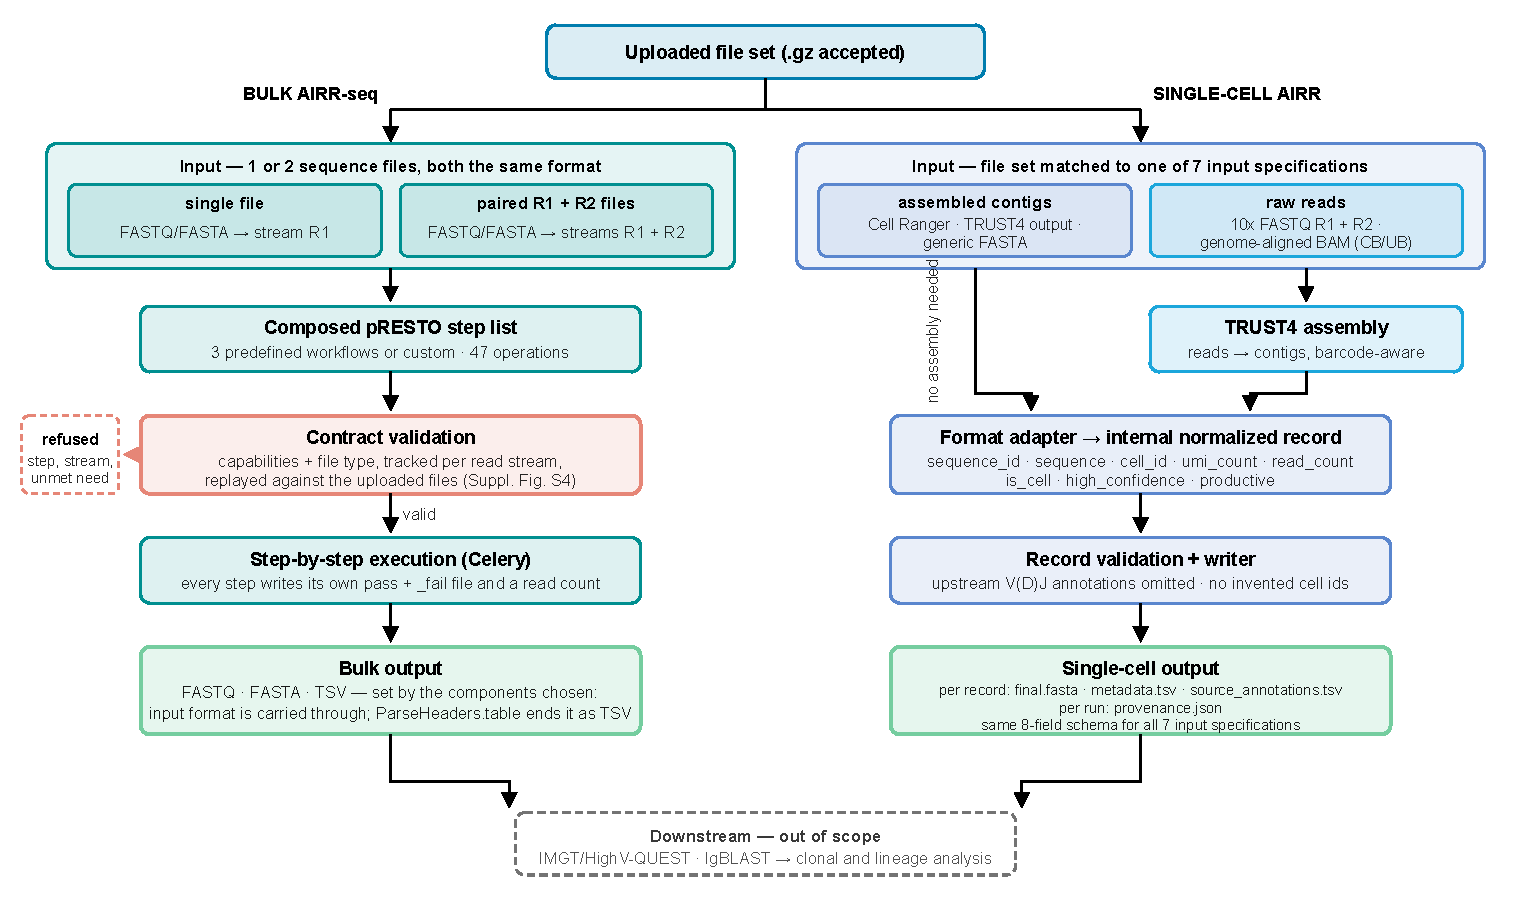
\includegraphics[width=0.94\textwidth]{figure1_workflow.pdf}
\caption{Overview of AIRRPrep. Bulk inputs are processed using predefined or custom pRESTO workflows whose computational compatibility is checked before execution. Single-cell inputs are normalized directly when reconstructed sequences are provided or are first assembled with TRUST4 when assembly is required. Every single-cell run writes three record-level outputs --- \texttt{final.fasta}, \texttt{metadata.tsv} and \texttt{source\_annotations.tsv}, keyed on the same \texttt{sequence\_id} --- plus the run-level \texttt{provenance.json}.}
\label{fig:workflow}
\end{figure*}

\subsection{Bulk workflow construction and pre-execution validation}
For bulk processing, AIRRPrep represents input as either one read stream from a FASTA or FASTQ file or separate R1 and R2 streams from matched paired-end files of the same format. Three predefined workflows reproduce documented pRESTO examples: UMI-barcoded MiSeq 2$\times$250 \citep{stern2014}, non-UMI MiSeq 2$\times$250 \citep{greiff2014} and UMI-barcoded 5$'$ RACE MiSeq 325+275 \citep{vanderheiden2017}; full parameters are listed in Supplementary Table~S9. A custom builder lets users compose workflows from 47 operations across 13 pRESTO tools (Supplementary Table~S2).
Each operation declares a contract specifying accepted file types, required and produced capabilities, companion files and read-stream behavior (Supplementary Figure~S4). Whereas pRESTO validates individual commands at execution, AIRRPrep propagates file type, available annotations and R1/R2 state through the proposed workflow beforehand. It rejects the first incompatible step and reports the affected step, stream and unmet requirement, such as quality filtering on FASTA or consensus generation before barcode annotation. The same contracts update which operations are selectable during construction and explain why others are disabled, guiding users toward workflows that are computationally coherent but not necessarily biologically appropriate (Supplementary Note~S1).
The interface also displays a count-annotated workflow graph, tracking R1 and R2 separately until assembly and the merged stream thereafter; the graph is exportable as a PNG (Supplementary Figures~S2 and~S3).

\subsection{Single-cell normalization}

Single-cell repertoire inputs contain receptor sequences together with cell-associated information, including cell barcodes, UMI counts and read support. AIRRPrep preserves these sequence-to-cell relationships while converting heterogeneous input formats into a unified representation for downstream repertoire analysis. Supported inputs include reconstructed outputs from Cell Ranger and TRUST4, as well as raw 10x FASTQ and genome-aligned BAM files (Supplementary Table~S1). When reconstructed sequences are provided, AIRRPrep directly parses and normalizes the existing output. For raw sequencing inputs, receptor assembly is first performed with TRUST4, followed by parsing and normalization of the resulting sequences and associated cell-level information. Format-specific adapters convert supported inputs into AIRRPrep's eight-field internal record, which is not an AIRR Rearrangement record. The run writes three record-level outputs --- \texttt{final.fasta} and \texttt{metadata.tsv}, which carry the receptor sequences and the associated metadata, including available cell identifiers, UMI counts and read support, and \texttt{source\_annotations.tsv} --- plus one run-level file, \texttt{provenance.json}. Missing values are preserved as empty fields rather than inferred, and cell identifiers are never generated from sequence identifiers alone. This approach maintains the link between each receptor sequence and its originating cell while providing a consistent structure across input sources. Upstream receptor annotations, including V(D)J gene calls, junctions and CDR3 annotations, are excluded from the normalized representation to enable consistent downstream annotation using a defined reference and procedure, such as IMGT/HighV-QUEST \citep{alamyar2012}. Available source annotations are retained separately in \texttt{source\_annotations.tsv}, one row per output record, keyed on the same \texttt{sequence\_id} as \texttt{final.fasta} and \texttt{metadata.tsv}. Processing information and checksums for the whole run are recorded in \texttt{provenance.json} (Supplementary Table~S1).

\subsection{Reproducibility and operation}
Workflow definitions can be exported for reuse, while completed runs provide exportable records of workflow structure, outputs and execution metadata. External companion files, such as primer FASTA inputs, are not embedded in workflow definitions; instead, required inputs are recorded with their file names, sizes and SHA-256 checksums. Exported records also include the software versions used during execution. Workflow graphs can be exported as images, allowing users to document the executed pipeline in manuscripts or reports. Long-running jobs can be recovered using email-based tracking without requiring a persistent user account (Supplementary Note~S2).

AIRRPrep uses a web-based client-server architecture with asynchronous job execution and state management through worker processes and Redis. The containerized environment includes TRUST4, BLAST+, samtools, MUSCLE, VSEARCH and CD-HIT and can be deployed on institutional infrastructure. The proprietary USEARCH is not included, and no predefined workflow depends on it. Software versions and execution dependencies are listed in Supplementary Table~S10.

\section{Validation}

The three predefined bulk workflows were evaluated against equivalent command-line pRESTO implementations using the first 25,000 read pairs from SRR4026043 \citep{vanderheiden2017}, ERR346600 \citep{greiff2014} and SRR1383456 \citep{stern2014}. Across all three workflows, AIRRPrep and pRESTO produced identical records, sequences, quality strings and annotations at each compared step; only record ordering differed (Supplementary Tables~S3--S5). Individual validation of the 47 supported operations showed equivalent output for 46 operations. The remaining \texttt{ConvertHeaders.py migec} case could not be directly compared because native pRESTO does not process the corresponding multi-record MIGEC input. The workflow validator accepted the predefined workflows and rejected invalid compositions involving missing annotations, incompatible file types, missing companion files and invalid read-stream states (Supplementary Note~S1).

Single-cell normalization was evaluated using Cell Ranger representations of the 10x Genomics \texttt{sc5p\_v2\_hs\_PBMC\_10k} T-cell V(D)J dataset. Normalized outputs matched the reference records without sequence, cell barcode, UMI, read count or cell-status discrepancies (Supplementary Table~S6). Generic FASTA inputs reproduced the same records when barcode mappings were provided, while inputs lacking a valid barcode mapping were rejected. TRUST4-based routes were evaluated using raw 10x reads and BAM inputs from the \texttt{sc5p\_v2\_hs\_PBMC\_1k} B-cell dataset, recovering all Cell Ranger-defined cells without assigning artificial cell identifiers (Supplementary Table~S7).

Execution time was evaluated on three replicates using identical pRESTO and Python environments on a Windows 11 workstation. AIRRPrep reduced execution time for the tested 25,000-read-pair workflows, primarily by avoiding repeated interpreter startup overhead between steps. Reference-guided assembly showed similar runtime between implementations because the underlying alignment operation dominated execution time. These measurements represent small-scale comparative execution tests on one workstation and are not intended as estimates of production-scale throughput.

\section{Discussion}

AIRRPrep simplifies access to established AIRR-seq preprocessing workflows while adding machine-checkable safeguards around workflow composition during construction and before execution. Stepwise record tracking makes runs auditable, and exported workflow definitions support reproducibility. Validation demonstrates computational coherence rather than biological appropriateness: a technically valid workflow can still contain unsuitable choices, such as an incorrect primer set or offset.

Runtime measurements represent small-input execution overhead on one Windows workstation and should not be interpreted as production-scale throughput benchmarks. Assembly and TRUST4 reconstruction remain the dominant computational steps in both implementations. AIRRPrep is intentionally focused on preprocessing: it does not perform germline assignment, and its single-cell output is an internal representation rather than an AIRR Rearrangement record \citep{vanderheiden2018}; therefore, AIRR compliance is not claimed. Future work will include cross-step quality-control summaries, support for additional single-cell platforms, resource-matched Linux benchmarks at production input sizes, and integration with downstream annotation tools.

\section*{Data availability}

AIRRPrep is available as a free hosted service at
\url{https://preprocessing.computimm.com}. The source code of the frontend and
backend, container definitions, automated tests, validation scripts and their
archived outputs (Supplementary Tables~S2--S7), together with the benchmark
scripts and results (Supplementary Tables~S8--S9), are publicly available at
\url{https://github.com/ComputImm/AIRRPrep} under the GNU Affero General
Public License v3.0 or later. The version described in this manuscript is
release \texttt{v1.0.0} (commit
\texttt{9148dba8bdd4c516b80db4eece07dd0a0b23a929}), archived at
\url{https://doi.org/10.5281/zenodo.22857985}. Large validation and benchmark
outputs that exceed repository limits are archived separately at
\url{https://doi.org/10.5281/zenodo.22858375}. The repository provides scripts
linking supplementary tables to the corresponding generated outputs and
includes SHA-256 checksums for archived files to support reproducibility.

Bulk validation used the first 25,000 read pairs from SRR4026043
\citep{vanderheiden2017}, ERR346600 \citep{greiff2014} and SRR1383456
\citep{stern2014}. Single-cell validation used Cell Ranger~5.0.0 outputs from
the 10x Genomics datasets \texttt{sc5p\_v2\_hs\_PBMC\_10k} and
\texttt{sc5p\_v2\_hs\_PBMC\_1k}. Input file checksums and validation outputs are
provided in Supplementary Tables~S6 and~S7. USEARCH is proprietary and is not
redistributed; the corresponding test commands, software version and results
are provided for users with an appropriate licence.

\section*{Author contributions}
Parsa Esmaeili: Conceptualization, Software, Validation, Writing --
original draft.
Fatemeh Chaker Hosseini Zavareh: Software, Methodology,
Validation, Data curation, Writing -- review \& editing.
Nika Abdolahi: Validation, Writing -- review \& editing.
Changiz Eslahchi: Conceptualization, Supervision,
Writing -- review \& editing.

\section*{Funding}
No specific funding was received for this work.

\section*{Conflict of interest}
None declared.

\begin{thebibliography}{9}

\bibitem[Vander Heiden et al.(2014)]{vanderheiden2014}
Vander Heiden JA, Yaari G, Uduman M, et al. pRESTO: a toolkit for processing high-throughput sequencing raw reads of lymphocyte receptor repertoires. \textit{Bioinformatics}. 2014;30(13):1930--1932.

\bibitem[Song et al.(2021)]{song2021}
Song L, Cohen D, Ouyang Z, Cao Y, Hu X, Liu XS. TRUST4: immune repertoire reconstruction from bulk and single-cell RNA-seq data. \textit{Nature Methods}. 2021;18:627--630.

\bibitem[Gabernet et al.(2024)]{gabernet2024}
Gabernet G, Marquez S, Bjornson R, et al. nf-core/airrflow: an adaptive immune receptor repertoire analysis workflow employing the Immcantation framework. \textit{PLoS Computational Biology}. 2024;20(7):e1012265.

\bibitem[Alamyar et al.(2012)]{alamyar2012}
Alamyar E, Duroux P, Lefranc M-P, Giudicelli V. IMGT/HighV-QUEST: the IMGT web portal for immunoglobulin and T cell receptor NGS repertoire analysis. \textit{Immunome Research}. 2012;8:26.

\bibitem[Christley et al.(2018)]{christley2018}
Christley S, Scarborough W, Salinas E, et al. VDJServer: a cloud-based analysis portal and data commons for immune repertoire sequences and rearrangements. \textit{Frontiers in Immunology}. 2018;9:976.

\bibitem[IJspeert et al.(2017)]{ijspeert2017}
IJspeert H, van Schouwenburg PA, van Zessen D, Pico-Knijnenburg I, Stubbs AP, van der Burg M. Antigen receptor Galaxy: a user-friendly, web-based tool for analysis and visualization of T and B cell receptor repertoire data. \textit{The Journal of Immunology}. 2017;198(10):4156--4165.

\bibitem[Vander Heiden et al.(2018)]{vanderheiden2018}
Vander Heiden JA, Marquez S, Marthandan N, et al. AIRR Community standardized representations for annotated immune repertoire data. \textit{Frontiers in Immunology}. 2018;9:2206.

\bibitem[Greiff et al.(2014)]{greiff2014}
Greiff V, Menzel U, Haessler U, et al. Quantitative assessment of the robustness of next-generation sequencing of antibody variable gene repertoires from immunized mice. \textit{BMC Immunology}. 2014;15:40.

\bibitem[Stern et al.(2014)]{stern2014}
Stern JNH, Yaari G, Vander Heiden JA, et al. B cells populating the multiple sclerosis brain mature in the draining cervical lymph nodes. \textit{Science Translational Medicine}. 2014;6(248):248ra107.

\bibitem[Vander Heiden et al.(2017)]{vanderheiden2017}
Vander Heiden JA, Stathopoulos P, Zhou JQ, et al. Dysregulation of B cell repertoire formation in myasthenia gravis patients revealed through deep sequencing. \textit{The Journal of Immunology}. 2017;198(4):1460--1473.

\end{thebibliography}

\end{document}
